% Lampiran Repositori Kode Sumber
\noindent
\begin{center}
	{\bfseries Lampiran Repositori Kode Sumber\par}
	\vspace{0.75em}

	\begin{tabular}{|p{0.25\textwidth}|p{0.65\textwidth}|}
		\hline
		\textbf{Nama Repositori} & EduTeams: Collaborative Team Formation System \\
		\hline
		\textbf{URL}             & \url{https://github.com/deymosxdeymos/equiteam} \\
		\hline
		\textbf{Deskripsi}       & Repositori kode sumber sistem EduTeams yang berisi implementasi lengkap aplikasi web pembentukan kelompok berbasis multi-faktor (MBTI, Skill, Gender, Preferensi Topik). \\
		\hline
		\textbf{Teknologi}       & Next.js, TypeScript, Prisma, PostgreSQL, Better Auth, Tailwind CSS \\
		\hline
	\end{tabular}
\end{center}
\refstepcounter{lampiran}%
\addcontentsline{app}{myappendices}{\protect\numberline{\thelampiran}Repositori Kode Sumber Sistem EduTeams}%
\begin{center}
	Lampiran~\thelampiran~Repositori Kode Sumber Sistem EduTeams
\end{center}
\label{fig:lampiran-repo}

\vspace{2em}

% Lampiran Wawancara Dosen
\begin{figure}[H]
	\centering
	{\bfseries Lampiran Wawancara Dosen\par}
	\vspace{0.75em}

	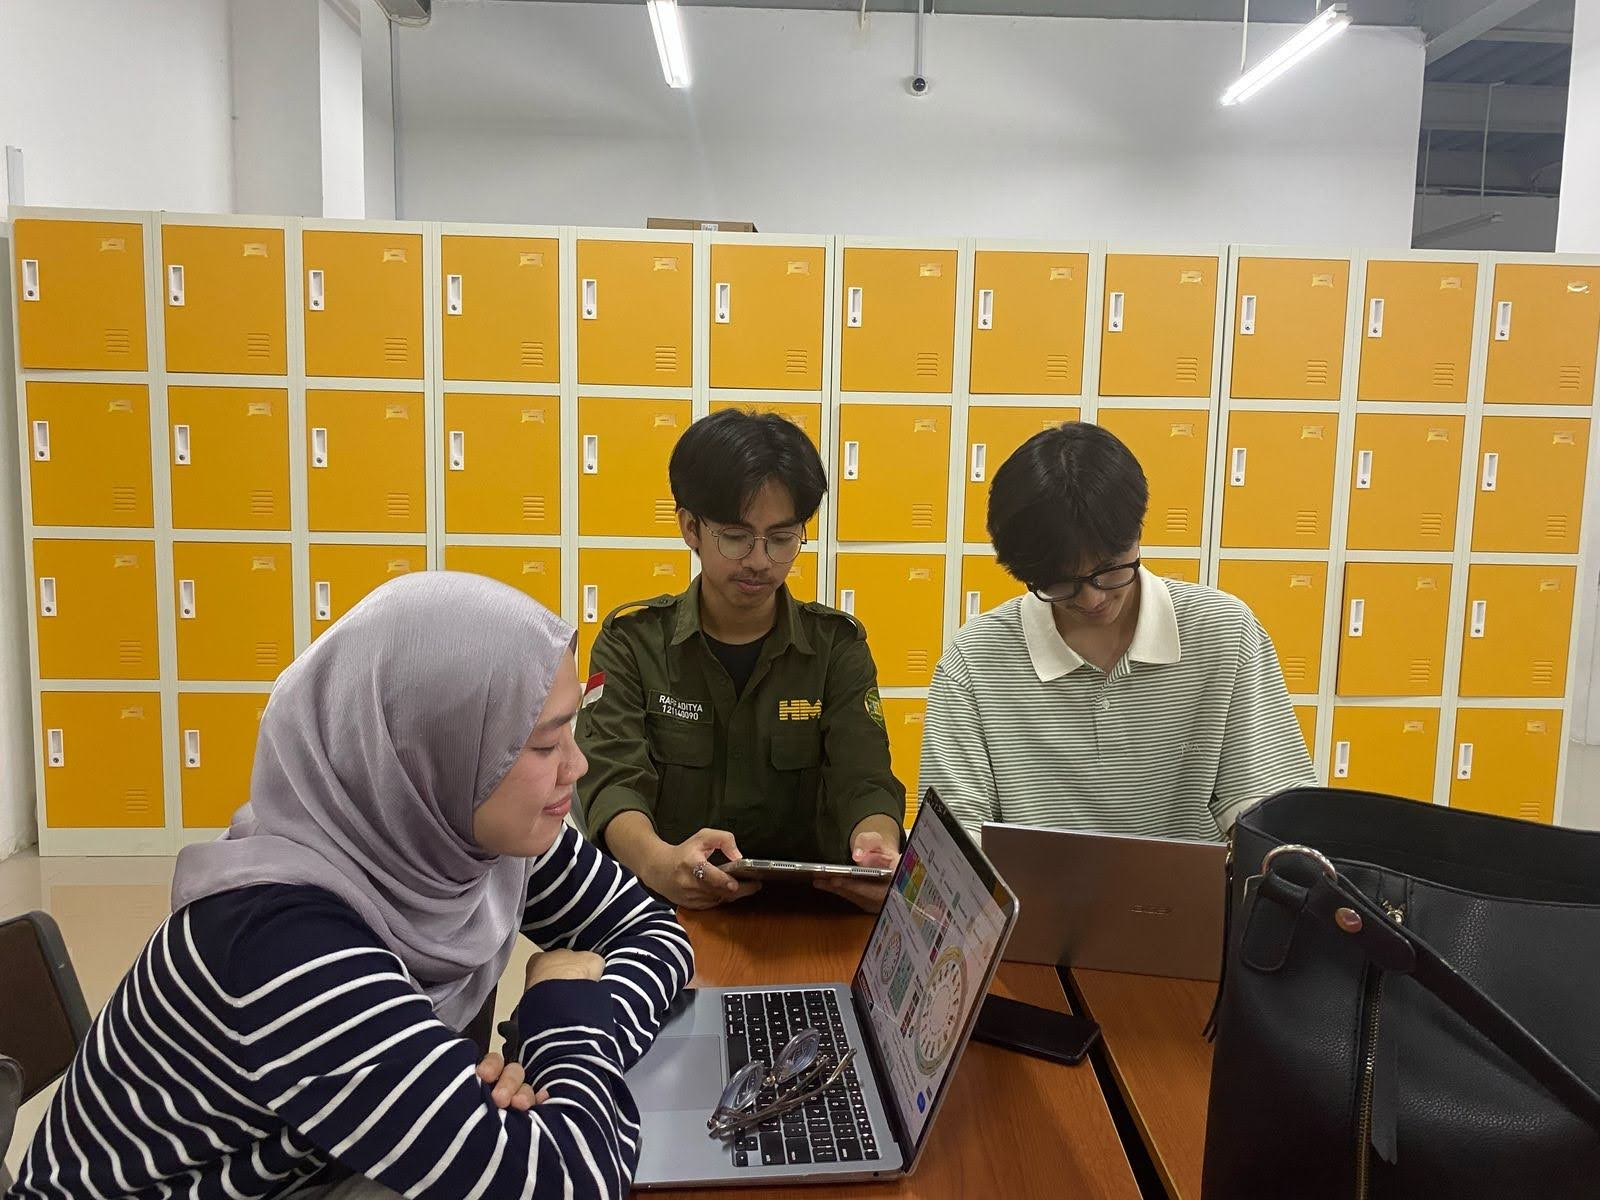
\includegraphics[height=0.35\textheight,keepaspectratio]{figure/lampiran/wawancara-dosen-1.jpg}
	\lampiran{Wawancara dosen 1}
	\label{fig:lampiran1}

	\vspace{1em}

	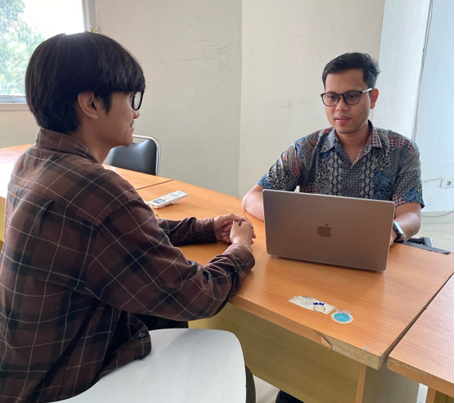
\includegraphics[height=0.35\textheight,keepaspectratio]{figure/lampiran/wawancara-dosen-2.png}
	\lampiran{Wawancara dosen 2}
	\label{fig:lampiran2}
\end{figure}

\begin{figure}[H]
	\centering
	{\bfseries Lampiran Wawancara Mahasiswa\par}
	\vspace{0.75em}

	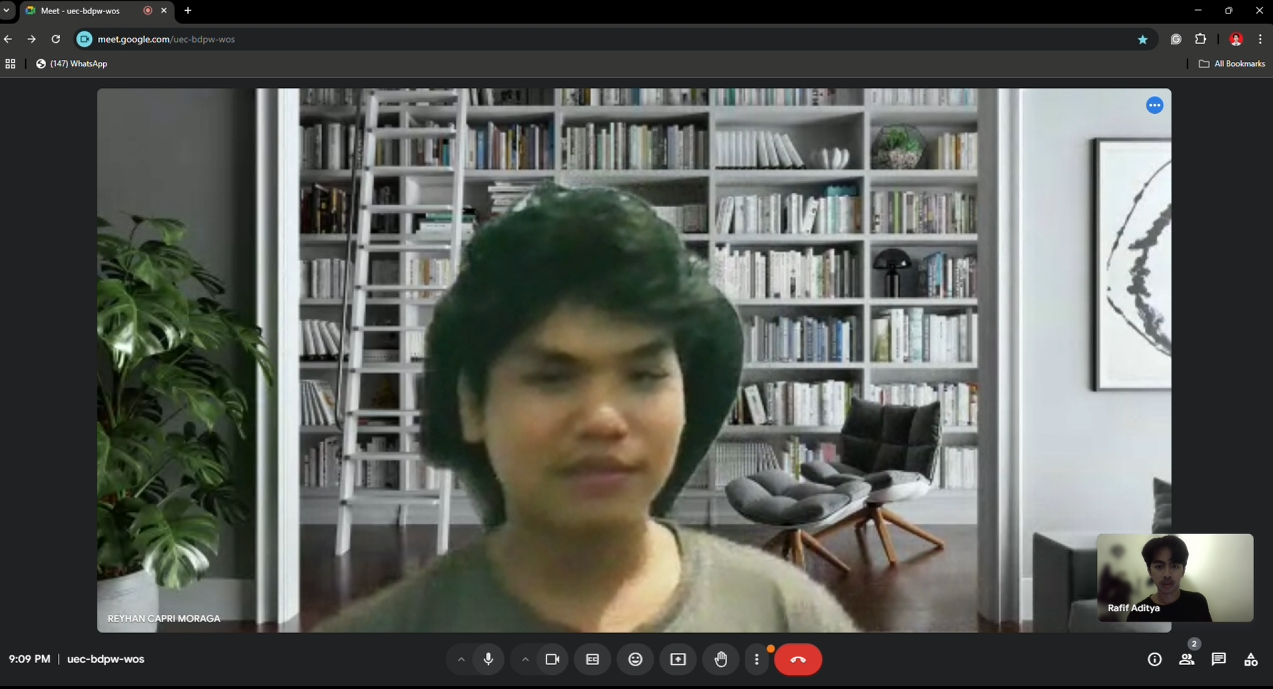
\includegraphics[width=0.8\textwidth]{figure/lampiran/wawancara-mahasiswa-1.png}
	\lampiran{Wawancara mahasiswa 1}
	\label{fig:lampiran3}
\end{figure}

\begin{figure}[h]
	\centering
	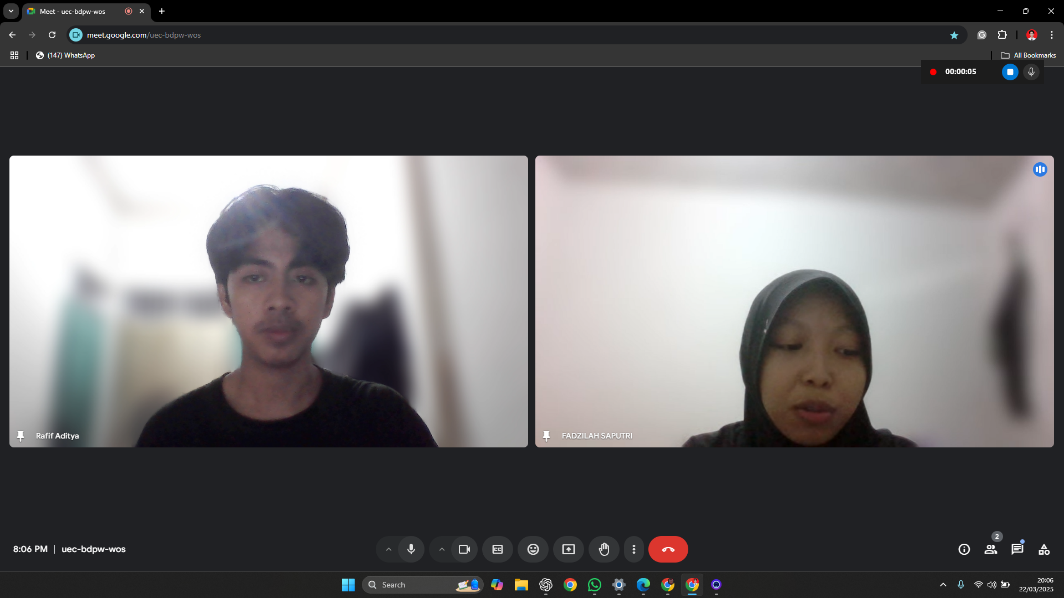
\includegraphics[width=0.8\textwidth]{figure/lampiran/wawancara-mahasiswa-2.png}
	\lampiran{Wawancara mahasiswa 2}
	\label{fig:lampiran4}
\end{figure}

\begin{figure}[h]
	\centering
	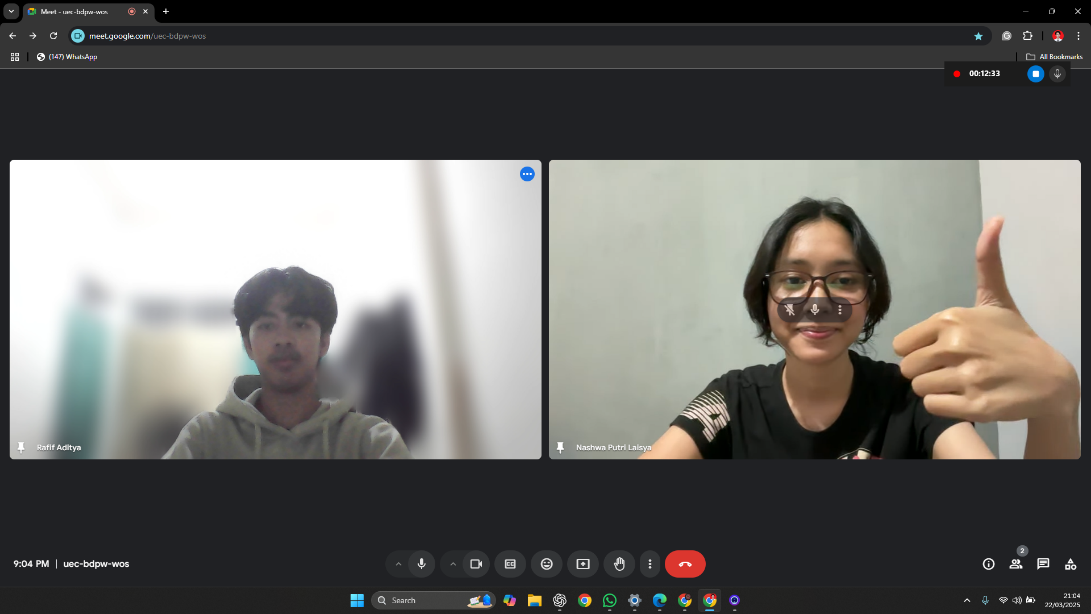
\includegraphics[width=0.8\textwidth]{figure/lampiran/wawancara-mahasiswa-3.png}
	\lampiran{Wawancara mahasiswa 3}
	\label{fig:lampiran5}
\end{figure}

\begin{figure}[h]
	\centering
	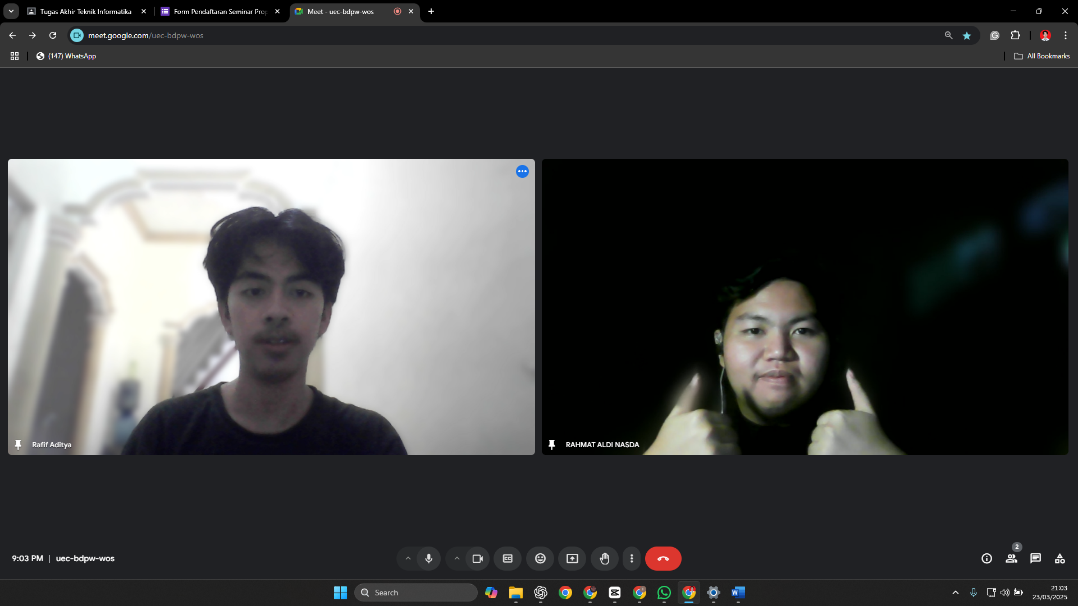
\includegraphics[width=0.8\textwidth]{figure/lampiran/wawancara-mahasiswa-4.png}
	\lampiran{Wawancara mahasiswa 4}
	\label{fig:lampiran6}
\end{figure}

\begin{figure}[h]
	\centering
	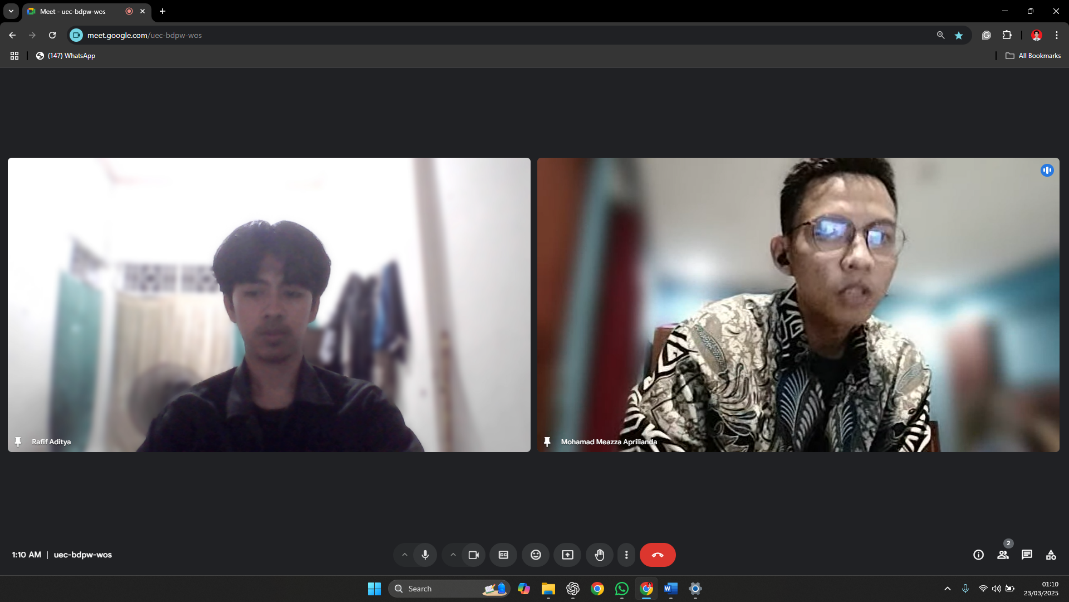
\includegraphics[width=0.8\textwidth]{figure/lampiran/wawancara-mahasiswa-5.png}
	\lampiran{Wawancara mahasiswa 5}
	\label{fig:lampiran7}
\end{figure}

\begin{figure}[h]
	\centering
	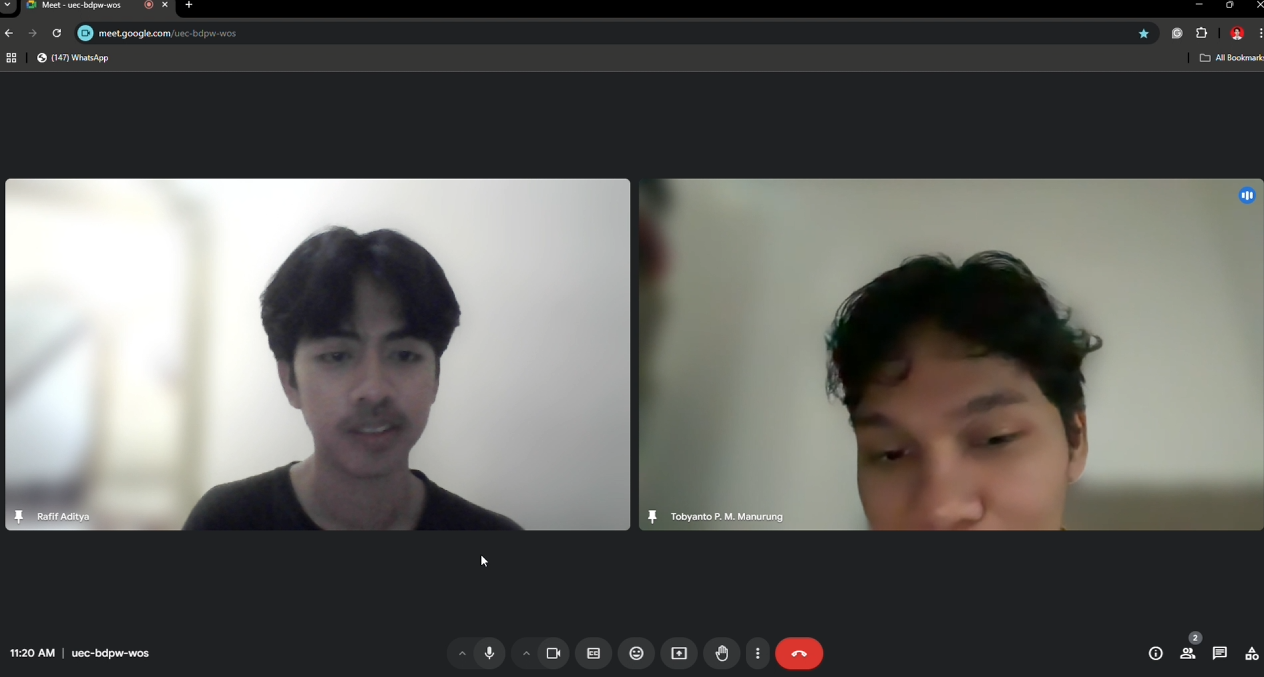
\includegraphics[width=0.8\textwidth]{figure/lampiran/wawancara-mahasiswa-6.png}
	\lampiran{Wawancara mahasiswa 6}
	\label{fig:lampiran8}
\end{figure}

\begin{figure}[h]
	\centering
	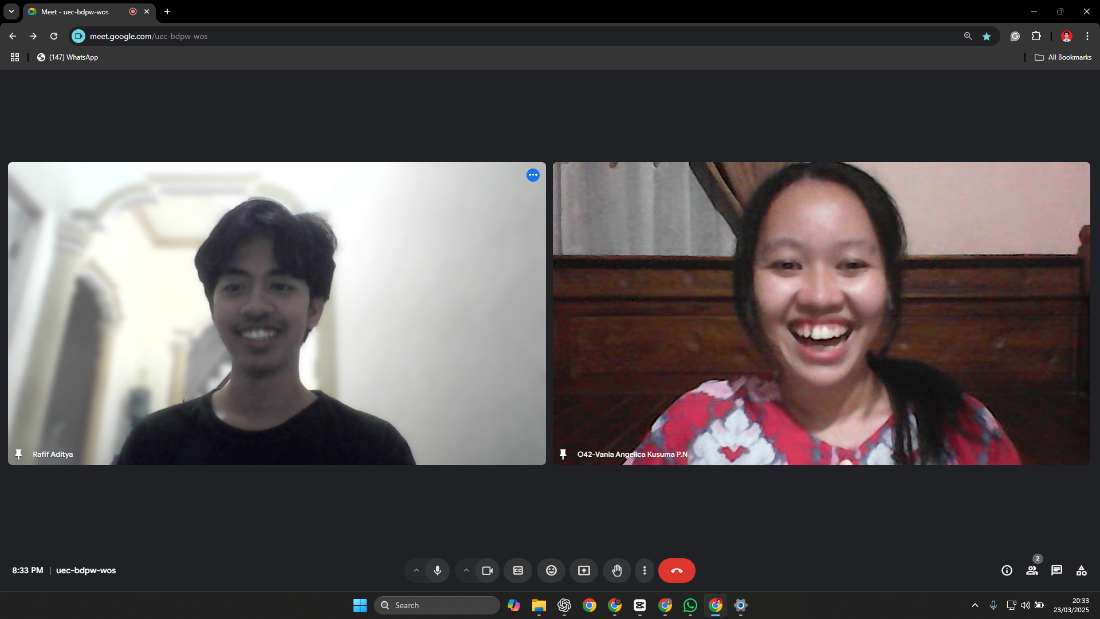
\includegraphics[width=0.8\textwidth]{figure/lampiran/wawancara-mahasiswa-7.png}
	\lampiran{Wawancara mahasiswa 7}
	\label{fig:lampiran9}
\end{figure}

\begin{figure}[h]
	\centering
	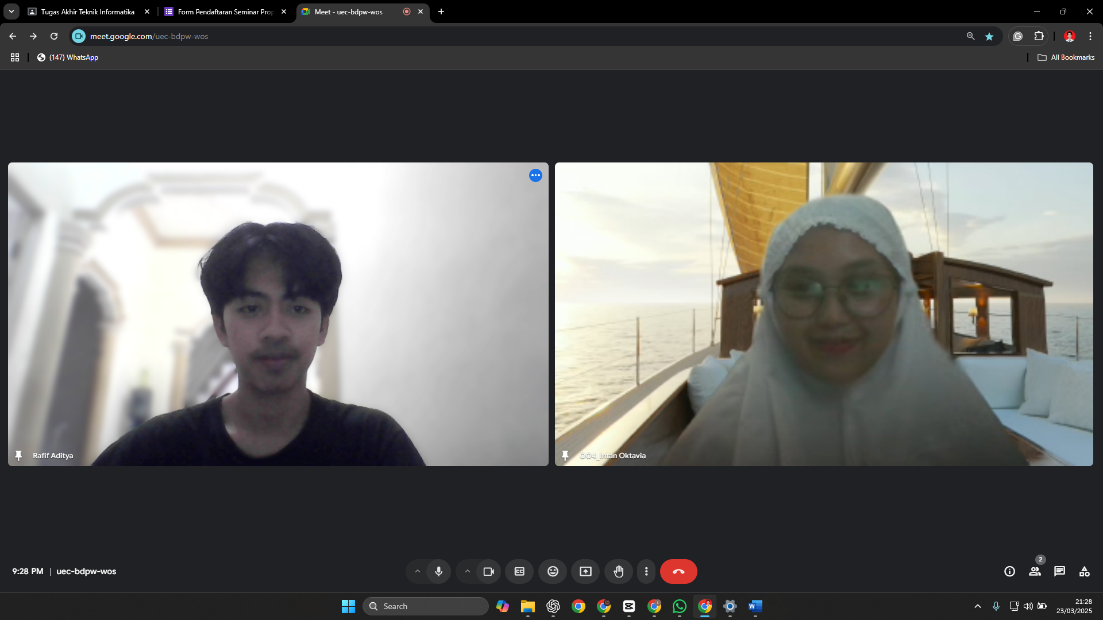
\includegraphics[width=0.8\textwidth]{figure/lampiran/wawancara-mahasiswa-8.png}
	\lampiran{Wawancara mahasiswa 8}
	\label{fig:lampiran10}
\end{figure}
